

\documentclass[journal]{IEEEtran}




\usepackage[pdftex]{graphicx}
% \graphicspath{{../pdf/}{../jpeg/}}
% \DeclareGraphicsExtensions{.pdf,.jpeg,.png}
\usepackage{amsmath}
\usepackage{booktabs}
\usepackage{amssymb}
\usepackage{wasysym}
\usepackage{listings}

%\usepackage{algorithmic}
%\usepackage{array}
%\usepackage{url}
% correct bad hyphenation here
\hyphenation{op-tical net-works semi-conduc-tor}

\usepackage{xcolor}
\usepackage{listings}
\lstset{basicstyle=\ttfamily,
	showstringspaces=false,
	commentstyle=\color{red},
	keywordstyle=\color{blue}
}

\usepackage{biblatex}
\usepackage[colorlinks=true,allcolors=black]{hyperref}
%\usepackage[backend=biber, bibencoding=utf8, style=ieee]{biblatex}
\addbibresource{references.bib}






\hyphenation{op-tical net-works semi-conduc-tor}


\begin{document}

\title{Assignment 3 - Phase 2: Using gem5 for estimating the performance of different application mappings onto different multi-core processors
}

\author{Snorri Steffanson, Filippo Bernardi,~\IEEEmembership{Master students,~TU Eindhoven}
}



% The paper headers
\markboth{Using gem5 to simulate application mapped onto different multi-core processors - S. Steffanson, F. Bernardi}%
{Shell \MakeLowercase{\textit{et al.}}: Bare Demo of IEEEtran.cls for IEEE Journals}


\maketitle

% As a general rule, do not put math, special symbols or citations
% in the abstract or keywords.
\begin{abstract}
Performance evaluation of the same application mapped onto different cores. The application is a Jpeg encoder program. The CPU used are an ARM A15-ARM A9 and a triple A9 cores. The program it has been divided used a profiler but also just by looking at the application itself. 
\end{abstract}

% Note that keywords are not normally used for peerreview papers.
\begin{IEEEkeywords}
ARM a9, ARM a15, gem5, multi threads, Valgrind 
\end{IEEEkeywords}




\IEEEpeerreviewmaketitle



\section{Introduction}

IEEEPARstart{T}{his} paper shows performance evaluation of the same application, a jpeg encoder, onto two different processors. Those two processors are composed differently. The first is a 3 ARM a9 core CPU. The second has one ARM a15 core and an ARM a9 core inside it.
On one hand, there is a CPU composed by an A9 core associated with a more powerful one. On the other hand, a CPU composed by balanced cores.
The first step done it was to analyze the given application. For this task, Valgrind program has been used.
The results is shown in figure \ref{fig:valgrind}

\begin{figure}[!h]
	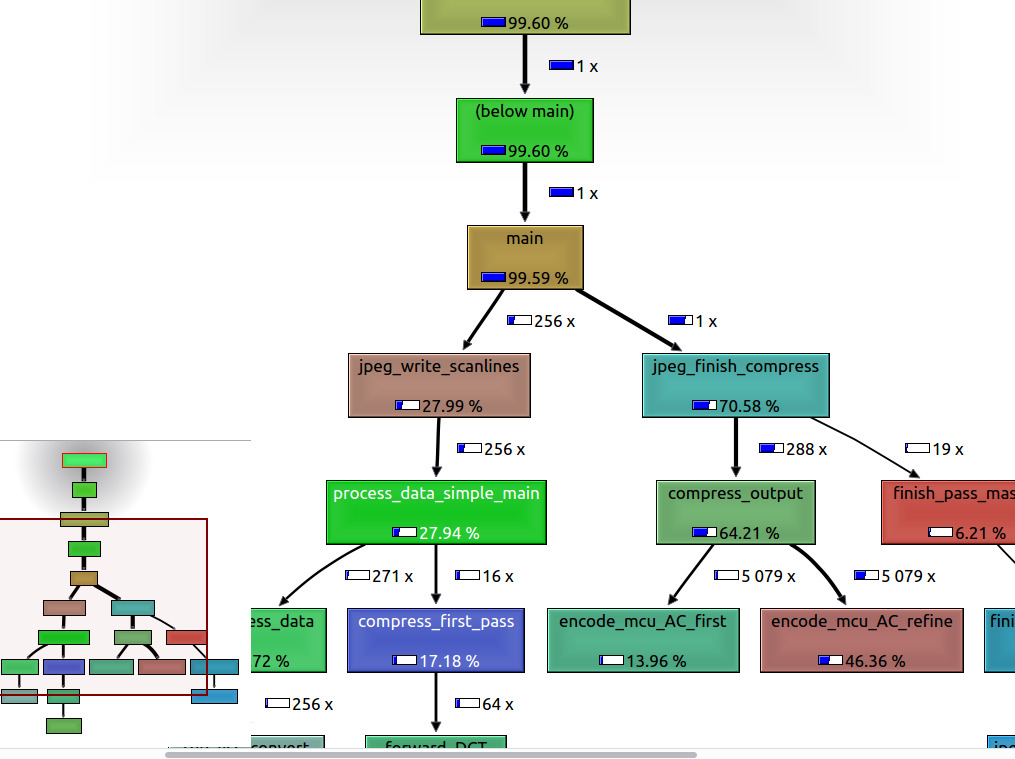
\includegraphics[width=\linewidth]{valgrind}
	\caption{Program calls in Valgrind}
	\label{fig:valgrind}
\end{figure}

This results gives the hint of divide the code inside the CPUs onto different cores, after the main function. This paper is divided onto different section, the first part concern the Gem5 simulator and Pthread library. The other section explains and evaluate different application results.\\

 
\hfill January 27, 2017


\section{Gem5 and Pthread library}
\subsection{Gem5 simulator}
Gem5 is the simulator used for testing the effectiveness and the results of the changes made on the code. The metric for evaluate the performances are the "tick". Tick are the results that gem5 displayed after every simulation and represent the total execution time in picoseconds. 
The simulator can both work in Full System mode and Syscall Emulation mode \(SE mode\). On one hand, in Full System mode the system it is much more accurate but it requires also a higher amount of time for run the simulation, in this case it is possible to boot an entire OS from scratch. On the other hand, in \(SE mode\) the system is less accurate but is much faster.
In this paper it is used only the \(SE mode\) because it is of interest evaluate an approximate results of the improved performance instead of an accurate analysis.
\subsection{Pthread library}
To divide the code into different threads, the Posix Thread library has been used.
The library is composed mainly by these three functions:

\begin{itemize}
	\item pthread\_create	
\begin{lstlisting}
int pthread_create(pthread_t * thread,
	const pthread_attr_t * attr,
	void * (*start_routine)(void *), 
	void *arg);
\end{lstlisting}

The function is needed to create new thread. 
The variable \(thread\) returns the thread ID. \(Attr\) it is possible to gives different attribute to the thread, set to NULL for default.
\(*start\_routine\) is the pointer to a function to be threaded. 
\(*arg\) is the argument to pass to the function. In order to pass multiple arguments, it is needed to create a struct and pass the struct as it has been done later on the report.\\


	\item pthread\_join
\begin{lstlisting}
int pthread_join(pthread_t th, 
	void **thread_return);
\end{lstlisting}
In this function a thread is suspended till \(th\) terminates. \(thread\_return\) return from the function.
This function it is used for waiting the end of a thread.
	\item pthread\_exit
\begin{lstlisting}
void pthread_exit(void *retval);
\end{lstlisting}
This terminate a thread, where \(*retval\) return the value of the function.
\end{itemize}
This description has been taken from\\
 \(http://www.yolinux.com/\)



\section{Function on thread}

What has been done firstly, is it try to run on the two architecture without change any code, the results have been the following:
23714598000 number of tick for the 3 a9 cores and 18786430000. 
Now, the jpeg finish compression has been placed in another thread, for doing so the following tutorial has been used: http://timmurphy.org/2010/05/04/pthreads-in-c-a-minimal-working-example/

On one thread the jpeg\_finish\_compress there are the same results for 3 a9 23641697000 and 21533576000 for a15-a9




\section{New application}
Due to the complexity of the jpeg compressing function we have decided to change to the same type of application but exploited in a simple manner. The new Program calls tree it can be seen in Figure \ref{fig:valgrind2}

\begin{figure}[!h]
	\centering
	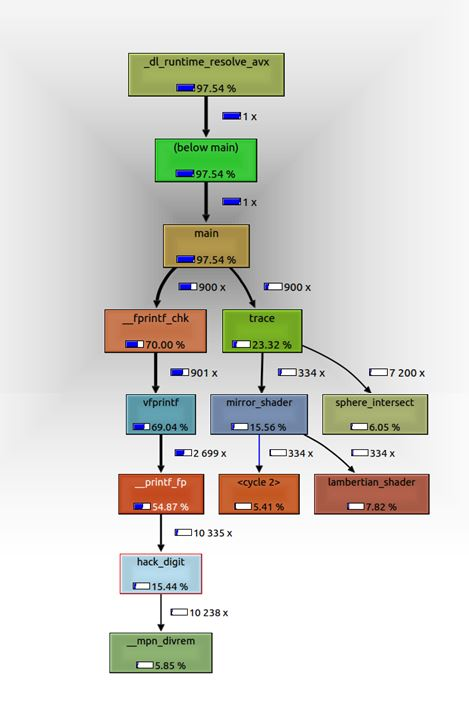
\includegraphics[width=.8\linewidth]{valgrind2}
	\caption{New jpeg application calls in Valgrind}
	\label{fig:valgrind2}
\end{figure}


\section{Pixels line on thread}
The final application threaten in this report has been inspired directly from the application itself. Moreover, instead of using Valgrind for dividing the code, the authors have questioned what the Jpeg compression was doing. On behalf of this, the code was possible to divide among the all pixels’ line that the function was making as output. Therefore, the line of the picture where divided into different thread. Multiple discussion has been created and reported on this section.
Firstly, a thread for each pixels’ line has been created. The idea was to created multiple thread and then let the compiler divide them among all the cores. 
To do so, it has been created a function pthread\_create for computing a line of the picture.
For doing so, a struct where all the variable needed to be passed to the thread, has been created:
\begin{lstlisting}
struct passToThread_struct{
int width_pixel;
float *res_0T,*res_1T,*res_2T;
scene_t *sceneT;
}f;
\end{lstlisting}
On the main, a normal iteration where left as it was on the code, then a new pixels’ line computation where created. After assign all the variable to pass, the pthread function where invoked:
\begin{lstlisting}
pthread_create(&col_thread_variable[px],
NULL, trace_thread, &f[px]);
\end{lstlisting} 
then the instance 
\begin{lstlisting}
pthread_join(col_thread_variable[px], 
NULL);
\end{lstlisting}
For join the thread to the main one.
The \(trace_thread\) function was created by adapting the code of the main used for calculate a line of pixel.\\

The code was now ready to be run using the script on the appendix.
However, because of gem5 was running in SE mode, it was not possible to create more thread that the cores available and then a different type of code has been created, tailored with the used CPU.
The results can be seen in figure \ref{fig:a9a9a9} for the 3 a9 processor, and in figure \ref{fig:a15a9} for the a15-a9 processor. As it is possible to see the overall performances where decreased of about 1\% and 2\% respectively.
As next step, the picture has been divided equally between the main and another thread. The result where already satisfactory with an increase in performance of 42\% in the 3 A9 processor and 17\% on the A15-A9 processor.\\

Finally, it has been created a different application for the two processors for use as much as possible the available resources. On the A15-A9 processor in fact, it has been allocated more pixel line on the first A15 core more powerful that the secondary A9. Splitting the code in 2/3 and 1/3 respectively for the A15 and A9 core the results was a 23\% of increase in overall performance.
On the other hand, for the triple A9 processor the application was slightly different: because the availability of the three cores, the thread created where three in this case. It has also been seen after some simulation and by printing on screen the order of execution of each pixel line, that the performance increase was much higher if instead of creating a balanced number of pixels’ line into each thread, was quite better to create an unbalanced one. In fact, we allocated 13 line on the first core, 6 on the second and 11 on the third one. The result was 58\% better in performance.





\begin{figure}[!h]
	\centering
	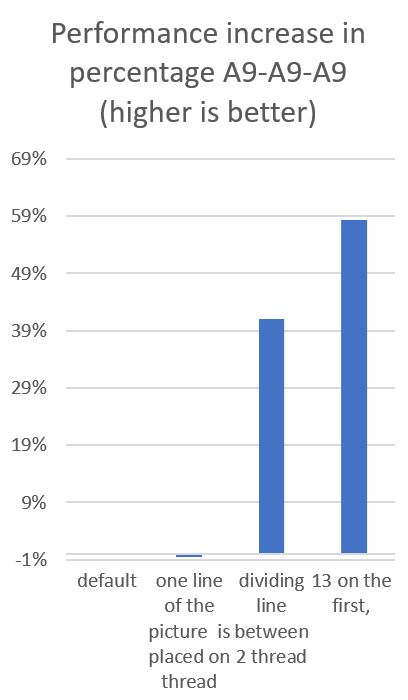
\includegraphics[width=.8\linewidth]{a9a9a9}
	\caption{Performances on a9 a9 a9 processor}
	\label{fig:a9a9a9}
\end{figure}

\begin{figure}[!h]
	\centering
	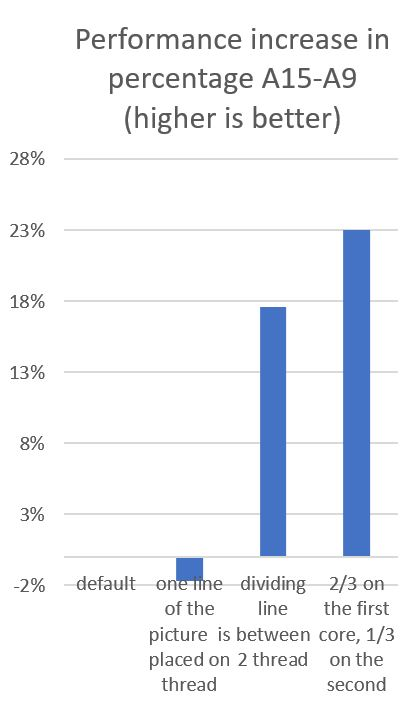
\includegraphics[width=.8\linewidth]{a15a9}
	\caption{Performances on a15 a9 processor}
	\label{fig:a15a9}
\end{figure}


\section{appendix}
\subsection{scripts}
\begin{lstlisting}
#!/bin/sh
cd /home/$USER/srt-clean
sudo rm callgrind.out.*
valgrind --tool=callgrind ./srt
kcachegrind callgrind.out.*
cd /
\end{lstlisting}

\begin{lstlisting}
#/bin/sh!
cd /home/$USER/srt-clean
make clean
make
cd /
\end{lstlisting}

\begin{lstlisting}
#/bin/sh!
cd /home/$USER/srt-clean
make clean
make -f Makefile.arm
/home/$USER/gem5/build/ARM/gem5.opt
/home/$USER/gem5/configs/example/arm-multic
	ore-A15-A9.py -c
	/home/$USER/srt-clean/srt
cd /
\end{lstlisting}

\begin{lstlisting}
#/bin/sh!
cd /home/$USER/jpeg/jpeg-6a/
make clean
make -f Makefile.arm
/home/$USER/gem5/build/ARM/gem5.opt
	 /home/$USER/gem5/configs/example/
	arm-multicore-A9-A9-A9.py -c 
	/home/$USER/srt-clean/srt
cd /
\end{lstlisting}


\begin{lstlisting}
#/bin/sh!
cd /home/$USER/srt-clean
make clean
make -f Makefile.arm
cd /
\end{lstlisting}



\section{Conclusion}
It is possible to conclude that the triple A9 has better performance that the A15-A9. This is true depending on how the program is divided onto the three or two cores. Moreover, there are cases where it is not possible to exploit parallelism, in this cases just one core is it used and the A15 one could win due to its characteristic. On the other hand, as in the Jpeg application, where parallelism was possible, it counts more the overall cores power in exploiting better performance. 
\end{document}


